\documentclass{article}

% NIPS style
\usepackage{nips12submit_e, times}

% figures
\usepackage{graphicx}
\graphicspath{{fig/}}

% links
\usepackage[hidelinks]{hyperref}

% better tables
\usepackage{booktabs}
\usepackage{multirow}
\newcommand{\ra}[1]{\renewcommand{\arraystretch}{#1}}


\title{Semi-Supervised Recursive Autoencoders}


\author{
Adrian Guthals \\
\texttt{aguthals@cs.ucsd.edu} \\
\And
David Larson \\
\texttt{dplarson@ucsd.edu} \\
}

\newcommand{\fix}{\marginpar{FIX}}
\newcommand{\new}{\marginpar{NEW}}

% don't show line numbers
\nipsfinalcopy 


\begin{document}

\maketitle


\begin{abstract}
We evaluate semi-supervised recursive autoencoders (RAE) as a method for predicting the sentiment of sentences. Using random word initialization and meaning vectors of length 20, we are able to predict the sentiment of a movie review dataset with a 74.5\% accuracy, which is only 3.3\% less than the 76.8\% accuracy reported in the 2011 paper ``Semi-Supervised Recursive Autoencoders'' by Soch et al.
\end{abstract}



%-----------------------------------------------------------------------------
% INTRO
%-----------------------------------------------------------------------------
\section{Introduction}
Learning the meaning of text documents, including short documents such as Twitter messages, is an active field of research in computer science. Until 2011, the state-of-the-art methods for predicting sentence-level meanings relied on either bag-of-words representations or manually generated resources, both of which have difficulty in dealing with complex sentiments. To overcome this shortcoming, Socher et al. introduced a new semi-supervised method based on neural networks \cite{Socher}. This study will attempt to recreate and expand upon the results reported in Socher et al.



%-----------------------------------------------------------------------------
% ALGORITHMS
%-----------------------------------------------------------------------------
\section{Recursive Autoencoders}
For any English sentence of length $n$, the syntactic structure of the sentence can be represented by a binary tree, where each word is a leaf node and the meaning of each node ($x$) is represented as a vector of length $d$ ($x \in R^d$) \cite{CSE250B}. A node that connects two or more words is a phrase, with its meaning being a function of its two children nodes. If node $k$ has children $i$ and $j$, then the meaning of node $k$ is:
\begin{equation}
    x_k = h(W[x_i ; x_j] + b)
    \label{eq:xk}
\end{equation}
where $W$ and $b$ are parameters to be learned while $h()$ is a pointwise sigmoid function which maps $R^d$ to $[-1, +1]^d$. As $x_k$, $x_i$, and $x_j$ are $\in R^d$, then $W \in R^{d \times 2d}$ and $b \in R^d$. To learn $W$ and $b$, the target meaning $t$ of the sentence must be known, which is usually not the case. To get around this, we use autoencoders, whose goal is to reconstruct the input \cite{CSE250B}.


%
% AUTOENCODERS
%
\subsection{Autoencoders}
For a node $k$ where $t$ is unknown, the inputs $z_i$ and $z_j$ of its children node meanings $x_i$ and $x_j$ can be approximated by:
\begin{equation}
    [z_i ; z_j] = U x_k + c
\end{equation}
where $x_k$ is the same as in Equation \ref{eq:xk}, and $U$ and $c$ are parameters to be learned ($U \in R^{2d \times d}$, $c \in R^d$). Then the square loss at node $k$ is:
\begin{equation}
    E = ||x_i - z_i||^2 + ||x_j - z_j||^2 = || [x_i;x_j] - U h(W[x_i; x_j] + b) - c||^2
\end{equation}
and the total loss of the tree is the sum of all errors at non-leaf nodes. Importance should be placed more on reduce the error of nodes that have more children nodes, which can be done by modifying the error function to:
\begin{equation}
    E_1 (k) = \frac{n_i}{n_i + n_j} ||x_i - z_i||^2 + \frac{n_j}{n_i + n_j} ||x_j - z_j||^2
\end{equation}
where $n_i$ and $n_j$ are the number of children nodes of nodes $i$ and $j$ respectively.


%
% TREE
%
\subsection{Binary Tree Construction}
If the tree structure of a sentence is unknown, it can be approximated using a greedy algorithm:
\begin{enumerate}
    \item calculate $E_1(k)$ for all $n - 1$ pairs of consecutive words
    \item select pair with minimum error and connect with a node
    \item calculate error for all possible pairs (now $n-2$ pairs)
    \item select pair with minimum error and connect with a node
    \item repeat until only one choice left for the root node
\end{enumerate}


%
% PREDICTING MEANINGS
%
\subsection{Predicting Labels using Meanings}
Although the target meaning is unknown, other target labels may be known, e.g., is the sentence positive or negative. If there are $r$ target labels, the probability of the labels at node $k$ can be found using multiclass logistic regress:
\begin{equation}
    \bar{p} = \textrm{softmax}(V x_k)
\end{equation}
where $V \in R^{r \times d}$ is a parameter matrix. The log loss of the predictions is therefore
\begin{equation}
    E_2 (k) = - \sum_{i=1}^r t_i \log p_i
\end{equation}
where $\bar{t}$ is the true label at node $k$ and is in $R^{r \times d}$.

To predict the target label for all internal nodes, excluding leaf nodes, we need to minimize the objective function $J$, which is defined as
\begin{equation}
    J = \frac{1}{m} \sum_{<s,t> \in S} E(s, t, \theta) + \frac{\lambda}{2} ||\theta||^2
\end{equation}
where $m$ is the length of each labelled training sentences in the set $S$, $\theta = < W, b, U, c, V >$ are the parameters to learn, $\lambda$ is the strength of $L_2$ regularization, and the total error for a sentence $s$ with a true label $t$ ($E(s, t, \theta)$) is
\begin{equation}
    E(s,t, \theta) = \sum_{k \in T(s)} \alpha E_1(k) + (1-\alpha) E_2(k)
\end{equation}
where $T(s)$ is the set of non-leaf nodes and $\alpha$ is a hyperparameter weighting the importance of the two per-node errors.


%
% BACKPROP
%
\subsection{Backpropogation}
Backpropogation is an efficient method for computing the derivatives required for training a neural network. Given



\subsection{Goal of Training}
The goal of training is to learn the parameters $\theta$ that minimize the objective function $J$.



\subsection{Gradient Verification}
It is important to verify the accuracy of the gradients calculated using backpropogation. For this study we have chosen to verify the accuracy of backpropogation by comparing against gradients calculated numerically using finite central-differences:
\begin{equation}
    \frac{\partial J}{\partial \theta} = \frac{J(\theta + \epsilon) - J(\theta - \epsilon)}{2\epsilon} + O(\epsilon ^2)
\end{equation}
where $\epsilon$ is the grid spacing.

A downside to using numerical derivatives to verify backpropogation is time complexity. If $W \in R^{2d \times d}$ then the time complexity of computing derivatives is $O(d^2)$ using backpropgation and $O(d^4)$ using finite central-differences, which is not feasible for real-world applications. One option for reducing the time complexity of checking the derivatives is to check a subset of the derivatives, chosen randomly, and assume those selected derivatives are representative of the entire set.


%-----------------------------------------------------------------------------
% EXPERIMENTS
%-----------------------------------------------------------------------------
\section{Experiments}

%
% DATASETS
%
\subsection{Datasets}
We use the same movie reviews dataset as in \cite{Socher}, which consists of 10662 snippets from reviews posted to the Rotten Tomatoes website\footnote{\url{http://www.rottentomatoes.com}}. Each snippet is roughly equivalent to a single sentence and includes a positive/negative label, with the entire dataset containing 5331 positive and 5331 negative labelled snippets. For all experiments we randomly selected 90\% of the original dataset as a training set, with the remaining 10\% used as a testing set. In splitting the dataset we have taken care to prevent any snippets from existing in both sets, so as to not contaminate the results.


%
% OPTIMIZATION
%
\subsection{Optimization}
We use limited-memory Broyden-Fletcher-Goldfarb-Shanno (L-BFGS), a well-known quasi-Newton optimization method, to learn the parameters $\theta$. Specifically we use the Matlab-based L-BFGS function from the minFunc toolbox \cite{minFunc} to minimize the objective function with parameters $\theta = < W, b, U, c, V>$ and gradient:
\begin{equation}
    \frac{\partial J}{\partial \theta} = \frac{1}{N} \sum_{(x, t)} \frac{\partial E(x, t; \theta)}{\partial \theta} + \lambda \theta
\end{equation}
where $N$ is the number of training examples.


%
% HYPERPARAMETERS
%
\subsection{Hyperparameters}
Due to time constraints, we evaluated the RAE model with $d=20$, instead of $d=100$ as in Socher et al. Also, we did not perform a grid search on $\alpha$ and $\lambda$, instead electing to use the same values as Socher et al. ($\alpha = 0.2$, $\lambda = <10^{-5}, 10^{-4}, 10^{-7}, 10^{-2}>$).

For the purpose of this study, we arbitrarily set $\epsilon = 10^{-4}$ and the maximum absolute error between the backpropogation and numerical derivatives to $10^{-6}$. 


%
% RANDOM INIT
%
\subsection{Random Word Initialization}
The meaning vector of each word was initialized randomly as in Socher et al. by using a Gaussian distribution of $\mu = 0$ and $\sigma ^2 = 0.05$.


%
% RESULTS
%
\subsection{Results}
With 10-fold cross-validation and $d=20$, we were able to achieve a prediction accuracy of 74.5\%. This is within 3\% of the prediction accuracy reported by Socher et al. (76.8\%). It should be noted that the accuracy reported by Socher et al. was for $d=100$, which indicates that there is a diminishing return after $d$ exceeds some threshold value.


\subsubsection{Most Positive and Negative}
Table \ref{tab:words}--\ref{tab:phrases} shows the words and phrases predicted to be the most positive and negative. The only result that stands out as possibly an error is the word ``flaws'' being predicted as positive rather than negative. Although the word ``flaws`` may be normally associated with a negative meaning, it could be associated with a positive meaning due its usage in a phrase, e.g., ``despite its flaws''.


\begin{table}[t]
    \centering

    \caption{Words predicted to be the most positive and negative.} 
    \label{tab:words}

    \ra{1.2}
    \begin{tabular}{@{} l l l @{}}
        \\
        \toprule
        \bf{Ranking} & \bf{Positive} & \bf{Negative} \\
        \midrule
        1 & beautiful   & fails  \\
        2 & brilliant   & boring \\
        3 & thoughtful  & neither\\
        4 & triump      & bad \\
        5 & flaws       & flat \\
        6 & beautifully & predictable \\
        7 & success     & bore \\
        8 & spectacular & poorly \\
        9 & enjoyable   & suffers \\
        10 & wonderful  & unnecessary \\
        \bottomrule
    \end{tabular}
\end{table}


\begin{table}[t]
    \centering

    \caption{Phrases (length 2) predicted to be the most positive and negative.} 
    \label{tab:phrases}

    \ra{1.2}
    \begin{tabular}{@{} l l l @{}}
        \\
        \toprule
        \bf{Ranking} & \bf{Positive} & \bf{Negative} \\
        \midrule
        1 & moving and      & lack of \\
        2 & an enjoyable    & boring .\\
        3 & and beautifully & how bad \\
        4 & a moving        & the dullest \\
        5 & a triumph       & flat , \\
        6 & a beautiful     & of bad \\
        7 & the best        & it fails \\
        8 & and powerful    & it isn't \\
        9 & its flaws       & and predictable \\
        10 & a wonderful    & a boring \\
        \bottomrule
    \end{tabular}
\end{table}


\subsubsection{Similar Meanings}
Comparing words and phrases with the most similar meanings is another intiutive method for evaluating the trained model. The similarity between a pair of words or phrases, with meaning vectors $x$ and $y$, can be quantified using cosine similarity:
\begin{equation}
    \textrm{cosine similarity} (x, y) = \frac{\sum_i x_i y_i}{\sqrt{\sum_i x_i^2} \sqrt{\sum_i y_i^2}}
\end{equation}
which is bounded between $-1$ (opposite in meaning) and $+1$ (same in meaning). Applying this metric to Table \ref{tab:words}--\ref{tab:phrases} we find the following pairs to be most similar:
\begin{enumerate}
    \item Positive words: ``bad'' and ``boring''
    \item Negative words: ``wonderful'' and ``enjoyable''
    \item Positive phrases (length 2): ``how bad'' and ``of bad''
    \item Negative phrases (length 2): ``moving and'' and ``and powerful''
\end{enumerate}


\subsubsection{Tree Structure of Interesting Sentences}
Visually inspecting the tree structure of sentences offers on insight on the strengths and weaknesses of the greedy algorithm. Figure \ref{fig:tree_positive} shows the structure of a positive sentence, which the greedy algorithm correctly determined. Meanwhile Figure \ref{fig:tree_negative} shows the structure of a negative sentence which the greedy algorithm performed poorly. Specifically, the structure should have connected ``right now'' with ``go , girls'' instead of ``the reality drain .''. Incorrectly determine tree structures such shown in Figure \ref{fig:tree_negative} likely caused problems for the RAE model and decreased it's prediction accuracy.


\begin{figure}[h]
\begin{center}
    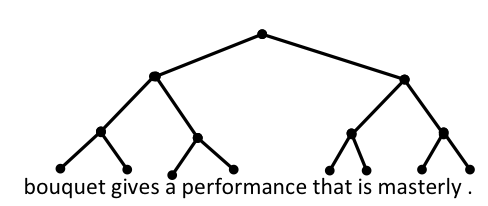
\includegraphics[width=0.7\textwidth]{tree_positive}
    \caption{The tree structured determined by the greedy algorithm of a positive sentence.}
    \label{fig:tree_positive}
\end{center}
\end{figure}


\begin{figure}[h]
\begin{center}
    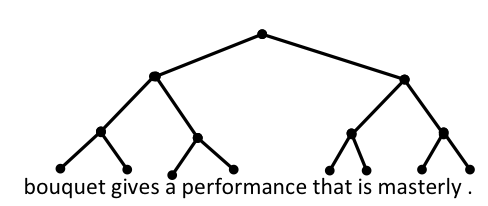
\includegraphics[width=0.7\textwidth]{tree_positive}
    \caption{The tree structured determined by the greedy algorithm of a negative sentence.}
    \label{fig:tree_negative}
\end{center}
\end{figure}




%-----------------------------------------------------------------------------
% CONCLUSION
%-----------------------------------------------------------------------------
\section{Conclusion}
Final remarks



%-----------------------------------------------------------------------------
% BIBLIOGRAPHY
%-----------------------------------------------------------------------------

\small{
\bibliographystyle{IEEEtran}
\bibliography{sources}
}



\end{document}
